\documentclass[conference]{IEEEtran}
\IEEEoverridecommandlockouts

\usepackage{cite}
\usepackage{amsmath,amssymb,amsfonts}
\usepackage{graphicx}
\usepackage{booktabs}
\usepackage{xcolor}
\usepackage{url}
\usepackage[hidelinks]{hyperref}
\graphicspath{{figures/}}

\begin{document}

\title{Remaining Useful Life Prediction for Turbofan Engines:\\
Sequence Models and a Hybrid Feature-Fusion Network}

\author{
\IEEEauthorblockN{Kushal Tyagi}
\IEEEauthorblockA{Enrollment No.\ 2401010249}
\and
\IEEEauthorblockN{Nishant Sharma}
\IEEEauthorblockA{Enrollment No.\ 2401010302}
\and
\IEEEauthorblockN{Anant Lalwani}
\IEEEauthorblockA{Enrollment No.\ 2401020086}
\and
\IEEEauthorblockN{Dev Tyagi}
\IEEEauthorblockA{Enrollment No.\ 2401010148}
\and
\IEEEauthorblockN{Vansh Khod}
\IEEEauthorblockA{Enrollment No.\ 2401010493}
\and
\IEEEauthorblockA{\textit{Newton School of Technology, Rishihood University}\\
Advanced Machine Learning $\cdot$ Project 7, Phase 2 (Deep Learning)}
}

\maketitle

\begin{abstract}
We compare models that learn remaining useful life (RUL) directly from sensor sequences with the engineered-feature regression of Phase~1 on NASA's C-MAPSS FD001 benchmark. A leakage-free pipeline turns every cycle into a 30-cycle window of 14 normalised sensors, keeps short histories through padding with a mask channel, and reuses Phase~1's engine-level folds. An LSTM, a temporal convolutional network and a Transformer encoder all learn real degradation patterns (test RMSE 14.7--15.5, against 18.2 for XGBoost on raw single-cycle sensors), but are significantly worse than XGBoost on 88 engineered features (10.75; paired Wilcoxon $p\leq0.0015$). Experiments trace the gap to information outside any fixed window: each engine's distance from its own healthy baseline, and its age. A hybrid network that fuses an LSTM encoder with the engineered features recovers the gap. It beats both of its branches and late fusion in cross-validation, is statistically level with XGBoost on the official benchmark (RMSE 11.02, $p=0.90$), and has the lowest error over all test cycles in every degradation stage. Ablations show that the features are the backbone ($+4.5$ RMSE without them) and that longer windows help sequence-only models but not the hybrid. Retraining with different seeds moves a CV score by about $\pm0.5$--$0.7$, so smaller design effects cannot be distinguished from training noise. Gradient saliency shows that the sequence branch relies on the core-speed sensors that the engineered features use least.
\end{abstract}

\begin{IEEEkeywords}
remaining useful life, C-MAPSS, LSTM, temporal convolutional network, Transformer, hybrid model, ablation study
\end{IEEEkeywords}

% Section owner: Kushal Tyagi -- introduction, sequence data and regularisation
\section{Introduction}
Remaining useful life (RUL) prediction estimates how many operating cycles an engine has left before it fails, from its multivariate sensor history~\cite{lei2018review}. Project~7 compares two routes on NASA's C-MAPSS FD001 benchmark~\cite{saxena2008damage,saxena2008dataset}: engineered degradation features with classical regression, and models that learn directly from sensor sequences.

Phase~1 built the first route. A leakage-free pipeline of 88 causal features (rolling statistics, trend slopes, deviation from each engine's own early-life baseline and a PCA health index) with XGBoost~\cite{chen2016xgboost} reached a test RMSE of 10.75 cycles. Its error analysis also identified where fixed-window features fall short: fast-degrading engines, the onset of degradation, and short histories. All three depend on the shape and timing of the full trajectory.

Phase~2 tests the second route and a combination of both. Our contributions are:
\begin{itemize}
  \item a sequence-data pipeline that keeps every cycle (including short histories, via padding and a mask channel) and is provably free of cross-engine and future leakage;
  \item an evaluation of the three architectures named in the brief, LSTM, temporal CNN and Transformer encoder, on the same engine-level folds as Phase~1;
  \item a hybrid feature-fusion network that combines a sequence encoder with the Phase~1 degradation features, justified by a specific blind spot of window-based models;
  \item ablation studies of branches, window length, regularisation and the padding mask;
  \item a validation on the official test set with three seeds, bootstrap confidence intervals, a paired significance test against Phase~1, stage-wise errors and gradient saliency.
\end{itemize}

% Section owner: Anant Lalwani -- deep learning deep learning literature
\section{Related Work: Deep Learning for RUL}
\textbf{Convolutional models.} Babu~\emph{et al.}~\cite{babu2016cnn} first applied a CNN to C-MAPSS sensor windows (FD001 RMSE 18.45). Li~\emph{et al.}~\cite{li2018dcnn} used a deeper 1-D CNN over 30-cycle windows with the piecewise-linear target and reported 12.61. Bai~\emph{et al.}~\cite{bai2018tcn} showed more generally that temporal convolutional networks (TCN) with causal, dilated convolutions, as introduced in WaveNet~\cite{oord2016wavenet}, and residual connections~\cite{he2016resnet} match or beat recurrent networks on many sequence tasks while training in parallel.

\textbf{Recurrent models.} The LSTM~\cite{hochreiter1997lstm} adds a gated, additively updated cell state to the recurrent network, so gradients survive over long sequences. Zheng~\emph{et al.}~\cite{zheng2017lstm} applied stacked LSTMs to C-MAPSS (FD001 RMSE 16.14), and Heimes~\cite{heimes2008rnn} had already used recurrent networks in the PHM'08 challenge.

\textbf{Attention.} The Transformer~\cite{vaswani2017attention} replaces recurrence with self-attention, relating every pair of time steps directly. Mo~\emph{et al.}~\cite{mo2021transformer} combined a Transformer encoder with a gated convolutional unit for RUL estimation on C-MAPSS.

\textbf{Hybrid models.} Al-Dulaimi~\emph{et al.}~\cite{aldulaimi2019hdnn} ran LSTM and CNN branches in parallel and fused them, and Chen~\emph{et al.}~\cite{chen2021attention} combined attention-based LSTM features with handcrafted features. Both support the idea of fusing complementary representations; our hybrid follows the second line, fusing a learned sequence representation with the engineered features of Phase~1. As in Phase~1, published numbers are indicative only, because preprocessing and evaluation protocols differ~\cite{ramasso2014benchmark}.

% Section owner: Kushal Tyagi -- sequence data and regularisation
\section{Sequence Data and Regularisation}\label{sec:data}
\subsection{Windows within engine boundaries}
For engine $i$ at cycle $t$, the model input is the window of the last $W$ cycles,
\begin{equation}
  X_{i,t}=\left[z_{i,t-W+1},\dots,z_{i,t}\right]\in\mathbb{R}^{W\times 14},
\end{equation}
where $z$ are the 14 informative sensors after the same z-score normalisation as Phase~1, fitted on training engines only. With stride one, every row of the data becomes one window (20{,}631 training windows), so both phases are trained and scored on exactly the same cycles. The target is the Phase~1 piecewise-linear RUL capped at 125~\cite{heimes2008rnn}, divided by 125 so that it lies in $[0,1]$.

\subsection{Short histories: padding and mask}
Cycles with fewer than $W$ predecessors are kept rather than discarded: the window is left-padded with the engine's own first reading, and a fifteenth channel marks real (1) and padded (0) steps. Without the mask, a padded window would look like a perfectly flat, healthy engine. With $W=30$, 14\% of training cycles and 22\% of test cycles have partly padded windows; at $W=80$ this rises to 38\% and 57\%, and 23 test engines are shorter than the window.

\subsection{Leakage control}
Three properties are checked in the notebook and in automated tests: (i) every window contains only its own engine's cycles (rebuilding each engine's windows in isolation gives identical arrays); (ii) windows are causal (deleting all future cycles leaves every remaining window unchanged, maximum difference $0$); (iii) normalisation statistics and the engineered features of the hybrid are refitted inside every fold.

\subsection{Splits}
We reuse Phase~1's five folds over engine ids (20 evaluation engines per fold), so CV scores are directly comparable across phases. Inside each fold, 10\% of the training engines are held out as an inner validation set for early stopping and the learning-rate schedule; the evaluation engines are never used for any training decision. The official test set is used once.

\subsection{Regularisation}
FD001 has only 100 training engines and consecutive windows overlap in $W-1$ cycles, so networks with tens of thousands of weights overfit quickly: in a demonstration run the inner-validation RMSE was lowest at epoch~10 and rose afterwards while the training error kept falling. We therefore combine dropout ($p=0.2$)~\cite{srivastava2014dropout}; decoupled weight decay ($\lambda=10^{-4}$) with the AdamW optimiser~\cite{kingma2015adam,loshchilov2019adamw}, i.e.\ minimising
\begin{equation}
  \mathcal{L}(w)=\frac{1}{n}\sum_{j}\left(\hat y_j(w)-y_j\right)^2+\lambda\lVert w\rVert_2^2;
\end{equation}
early stopping with patience 8 and restoration of the best weights~\cite{prechelt1998early}; halving the learning rate on validation plateaus; and gradient-norm clipping at 1.0, which protects recurrent networks from exploding gradients~\cite{pascanu2013difficulty}. Gaussian input noise ($\sigma=0.05$) is evaluated as an augmentation in the ablations.

% Section owner: Anant Lalwani -- sequence architectures
\section{Sequence Architectures}\label{sec:arch}
All three networks map a window $X\in\mathbb{R}^{30\times 15}$ to an embedding $h$, followed by the same head (32 ReLU units, dropout, one linear output).

\textbf{LSTM.} Two stacked layers of 64 units read the window cycle by cycle:
\begin{equation}
\begin{aligned}
f_t&=\sigma(W_f[h_{t-1},x_t]+b_f),\quad i_t=\sigma(W_i[h_{t-1},x_t]+b_i),\\
c_t&=f_t\odot c_{t-1}+i_t\odot\tanh(W_c[h_{t-1},x_t]+b_c),\\
h_t&=\sigma(W_o[h_{t-1},x_t]+b_o)\odot\tanh(c_t).
\end{aligned}
\end{equation}
The forget and input gates decide what the cell state keeps and adds; because $c_t$ is updated additively, the gradient along it does not shrink geometrically with the sequence length. The final hidden state is the embedding (56k parameters).

\textbf{TCN.} Residual blocks of two causal 1-D convolutions (kernel $k=3$, 64 channels) with dilations $d_l=1,2,4,8$ give a receptive field
\begin{equation}
R=1+\sum_l 2(k-1)\,d_l=61\ \text{cycles}\geq W.
\end{equation}
Causality (left padding only) guarantees that the output at cycle $t$ uses no later input; the embedding is the output at the last cycle (93k parameters).

\textbf{Transformer encoder.} Inputs are projected to width 64, sinusoidal positional encodings are added, and two pre-norm encoder layers with four heads apply
\begin{equation}
\mathrm{Attention}(Q,K,V)=\mathrm{softmax}\!\left(QK^\top/\sqrt{d_k}\right)V,
\end{equation}
with padded steps removed from attention by the mask. The output at the current cycle is the embedding (70k parameters).

\subsection{Cross-validation results}
Table~\ref{tab:seq} compares the three networks with the Phase~1 models on the same folds. All networks beat XGBoost on single-cycle raw sensors (18.57) by 3 to 5.5 cycles, so learning from the 30-cycle history is clearly useful. The Transformer is best ($13.05\pm0.73$), followed by the LSTM and the TCN. None reaches the engineered-feature XGBoost (9.26). Their errors are largest in the onset region (RUL 60--100, up to 20 cycles for the Transformer against 13--15 for XGBoost), where the drift within 30 cycles is small compared with the noise. The likely reason is that a 30-cycle window cannot see the engine's own healthy baseline or its age, the two most important pieces of information in Phase~1, and 100 engines are too few for a network to learn such long-range references from scratch.

\begin{table}[t]
\centering
\small
\caption{5-fold CV RMSE (capped target, same folds as Phase 1)}
\label{tab:seq}
\begin{tabular}{lcc}
\toprule
Model (input) & RMSE (mean $\pm$ std) & MAE \\
\midrule
XGBoost (raw, one cycle) & 18.57 $\pm$ 0.53 & 13.49 \\
TCN (window) & 15.41 $\pm$ 0.95 & 11.65 \\
LSTM (window) & 14.01 $\pm$ 1.23 & 10.20 \\
Transformer (window) & 13.05 $\pm$ 0.73 & 8.74 \\
XGBoost (88 features) & \textbf{9.26 $\pm$ 0.50} & \textbf{6.30} \\
\bottomrule
\end{tabular}
\end{table}

\begin{figure}[t]
  \centering
  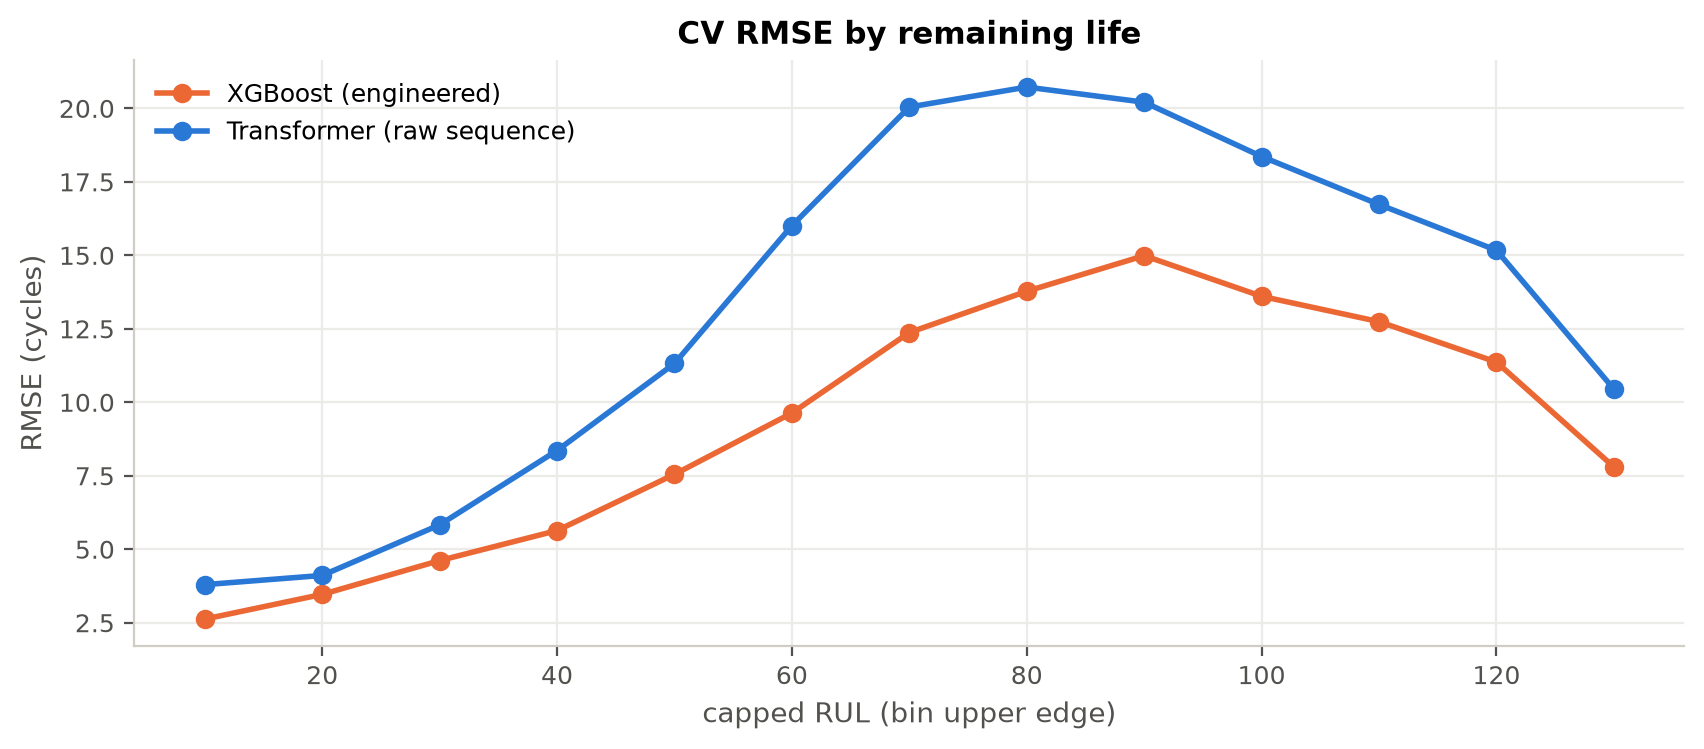
\includegraphics[width=\columnwidth]{07_error_by_rul.png}
  \caption{CV RMSE by remaining life: the sequence model's gap to XGBoost is largest at the onset of degradation.}
  \label{fig:bins}
\end{figure}

% Section owner: Nishant Sharma -- hybrid feature-fusion model
\section{Hybrid Feature-Fusion Model}\label{sec:hybrid}
\subsection{Rationale}
The two routes see an engine differently, and each misses what the other has. The engineered features summarise information that lies \emph{outside} any fixed window, most importantly the distance of each sensor from the engine's own first ten cycles, which Phase~1 found to be the most informative feature group, and the engine's age. A window-based network cannot compute these, because the first cycles of a long-lived engine are not in its 30-cycle window. Conversely, the features compress the recent history into a few hand-chosen statistics and cannot represent trajectory shapes that the designer did not anticipate. Section~\ref{sec:arch} showed the cost of the first gap: the networks fall 4--6 cycles behind XGBoost, most of all at the onset of degradation. A hybrid that gives the network both views addresses this specific blind spot, which is the ``degradation feature engineering $\rightarrow$ sequence-based prediction'' logic of the project brief.

\subsection{Architecture}
\begin{equation}
\begin{aligned}
h_{\text{seq}}&=\mathrm{Enc}(X_{i,t}),\qquad h_{\text{feat}}=\mathrm{MLP}(f_{i,t}),\\
\hat y_{i,t}&=g\!\left([h_{\text{seq}};h_{\text{feat}}]\right),
\end{aligned}
\end{equation}
where $\mathrm{Enc}$ is one of the three encoders of Section~\ref{sec:arch} (64-d output), $f_{i,t}$ are the 88 standardised Phase~1 features at cycle $t$ (causal, refitted per fold), the MLP is $88\rightarrow64\rightarrow32$ with ReLU and dropout, and $g$ is $96\rightarrow64\rightarrow1$. Both branches are trained jointly with one loss, so the encoder is pushed to learn what the features do not already explain. This \emph{early} (feature-level) fusion differs from averaging two separately trained models (\emph{late} fusion), which we test as a baseline.

\begin{figure}[t]
  \centering
  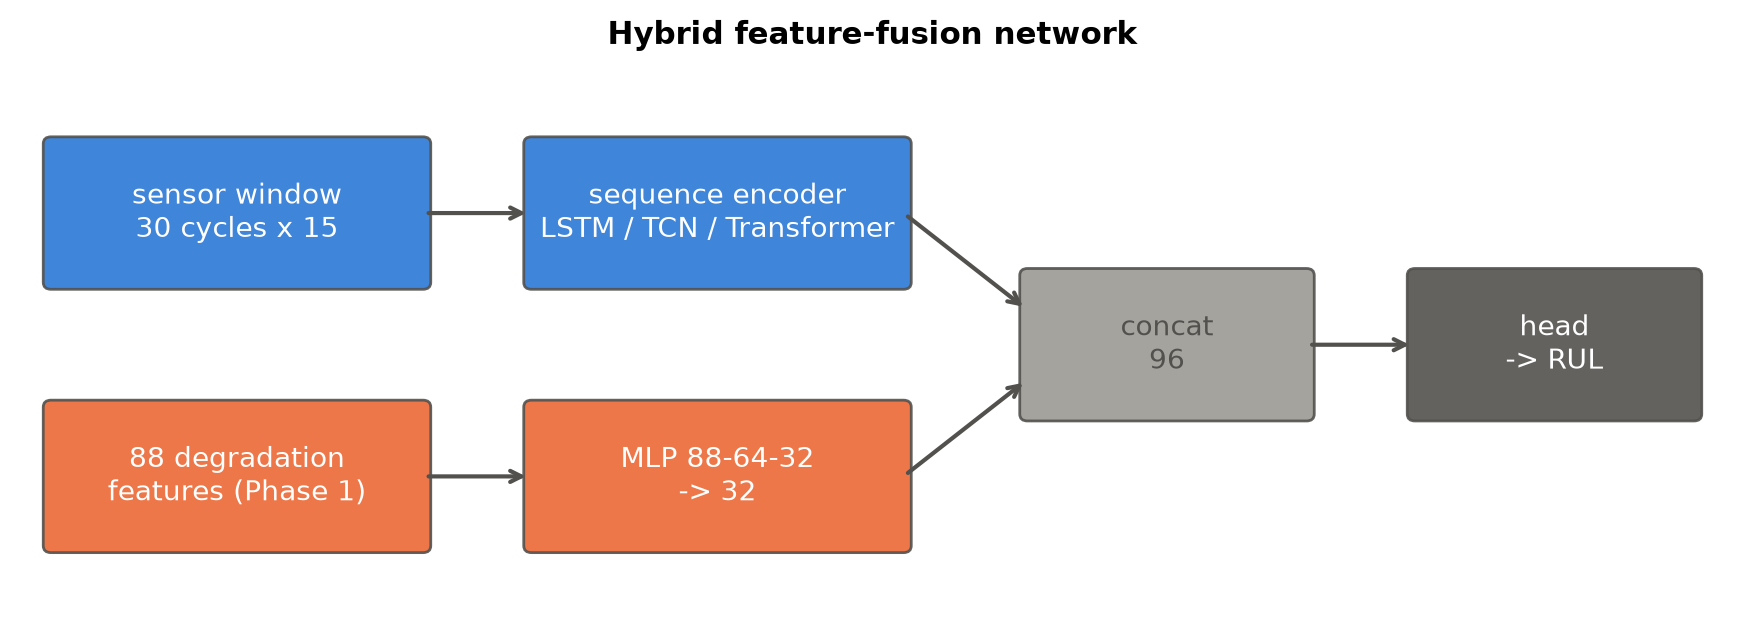
\includegraphics[width=\columnwidth]{08_hybrid_architecture.png}
  \caption{Hybrid feature-fusion network.}
  \label{fig:hybrid}
\end{figure}

\subsection{Results}
Table~\ref{tab:hybrid} reports the hybrid against its two branches, Phase~1's XGBoost, and the late-fusion average. With the LSTM encoder, the hybrid ($9.55\pm0.77$) is 4.5 cycles better than the best sequence model alone and 0.5 cycles better than the feature branch alone, so each branch contributes information. Joint training matters: averaging XGBoost and the Transformer scores 10.24, worse than XGBoost alone, while the hybrid beats the average with every encoder. Against XGBoost (9.26) the hybrid is close but not better: it wins on 2 of 5 folds, and averaged over three seeds (Section~\ref{sec:ablation}) its CV RMSE is about 9.7--10.0.

The gain is concentrated where it matters most. In the last 50 cycles before failure the hybrid's RMSE is 4.14 against 5.04 for XGBoost (18\% lower) and 7.20 for the Transformer alone. In the onset region it recovers almost all of the sequence model's weakness (14.31 vs.\ 19.07; XGBoost 13.80). Fast-degrading engines remain about 10 cycles late for both XGBoost and the hybrid, since both use the engine's age, which makes a fast degrader look too young to fail.

\begin{table}[t]
\centering
\small
\caption{Hybrid versus its parts (5-fold CV RMSE)}
\label{tab:hybrid}
\resizebox{\columnwidth}{!}{\begin{tabular}{lcc}
\toprule
Model & RMSE & RMSE, last 50 cycles \\
\midrule
Sequence alone (Transformer) & 13.05 & 7.20 \\
Feature branch alone (MLP) & 10.04 & -- \\
Average of XGBoost and Transformer & 10.24 & -- \\
XGBoost, engineered (Phase~1) & \textbf{9.26} & 5.04 \\
Hybrid, TCN encoder & 9.87 & -- \\
Hybrid, Transformer encoder & 9.74 & -- \\
Hybrid, LSTM encoder & 9.55 & \textbf{4.14} \\
\bottomrule
\end{tabular}}
\end{table}

% Section owner: Dev Tyagi -- ablation studies
\section{Ablation Studies}\label{sec:ablation}
Each ablation changes one component of the LSTM hybrid and keeps everything else fixed (folds, inner validation engines, seed). Table~\ref{tab:ablation} and Fig.~\ref{fig:ablation} report the change in 5-fold CV RMSE. Before interpreting them, we measured how much a CV score moves when the \emph{same} configuration is retrained with different seeds (Table~\ref{tab:seeds}): about $\pm0.5$--$0.7$ cycles. Re-running one ablation with an identical configuration also gave 9.39 and then 9.60, because parallel floating-point arithmetic on a multi-core CPU is not bit-reproducible. We therefore treat only effects clearly larger than about 0.5 cycles as established.

\textbf{Branches.} Removing the feature branch costs $+4.46$ cycles (worse on all five folds), far beyond the noise: the engineered features are the backbone. Removing the sequence branch costs $+0.49$ (worse on four of five folds). That is consistent across folds but of the same size as seed noise, so the value of the sequence branch rests on several pieces of evidence together: this ablation, the stage-wise test results (Section~\ref{sec:test}) and the saliency analysis.

\textbf{Window length.} This ablation tests the Phase~1 hypothesis that fixed windows miss long degradation trajectories, and it is the clearest result. For the LSTM \emph{alone}, a longer history helps markedly: RMSE falls from 14.01 ($W=30$) to 11.87 ($W=50$), then rises to 12.46 at $W=80$, where 38\% of training cycles become partly padded. The hybrid barely changes (9.55, 9.49, 9.51), because its engineered features already carry the long-range context. We keep $W=30$, which gives the same accuracy at a fraction of the cost (3 versus 44 minutes of CV training at $W=80$).

\textbf{Regularisation and mask.} Dropout ($+0.12$ without it), weight decay ($-0.03$), Gaussian input noise ($+0.05$) and the padding mask ($+0.18$ without it) all change the error by less than the seed noise, so none of them can be shown to matter on its own at this data size. Early stopping is different. Its signal comes from only 7--8 inner-validation engines, and it stopped at epochs 14--30. Trained for a fixed 60 epochs, the hybrid's validation error ends within 0.05--0.4 cycles of its best value on every fold, so dropout and the learning-rate schedule are enough to prevent overfitting. For the sequence-only networks, whose validation error turned up after 7--16 epochs, early stopping remains necessary.

\textbf{Final configuration.} A single run with a fixed 60 epochs gave the lowest CV RMSE (9.20). Over three seeds, it remains better and steadier than the default ($9.73\pm0.54$ vs.\ $9.99\pm0.71$), and it was adopted for the test evaluation. The choice used only the CV folds. Averaged over seeds, the hybrid's CV RMSE is slightly behind XGBoost (9.26).

\begin{table}[t]
\centering
\small
\caption{Ablations of the LSTM hybrid (5-fold CV RMSE, one seed)}
\label{tab:ablation}
\resizebox{\columnwidth}{!}{\begin{tabular}{lcc}
\toprule
Variant & RMSE & $\Delta$ vs.\ hybrid \\
\midrule
Hybrid ($W=30$, early stopping) & 9.55 & -- \\
\midrule
Without sequence branch & 10.04 & $+0.49$ \\
Without feature branch & 14.01 & $+4.46$ \\
$W=50$ / $W=80$ & 9.49 / 9.51 & $-0.06$ / $-0.04$ \\
Without dropout & 9.67 & $+0.12$ \\
Without weight decay & 9.52 & $-0.03$ \\
Fixed 60 epochs (no early stopping) & \textbf{9.20} & $-0.36$ \\
With input noise ($\sigma=0.05$) & 9.60 & $+0.05$ \\
Without padding mask & 9.74 & $+0.18$ \\
\bottomrule
\end{tabular}}
\end{table}

\begin{table}[t]
\centering
\small
\caption{Seed variability of the hybrid's CV RMSE}
\label{tab:seeds}
\resizebox{\columnwidth}{!}{\begin{tabular}{lcccc}
\toprule
Configuration & seed 42 & seed 1 & seed 2 & mean $\pm$ std \\
\midrule
Early stopping (default) & 9.55 & 10.81 & 9.61 & $9.99\pm0.71$ \\
Fixed 60 epochs (final) & 9.20 & 10.27 & 9.71 & $\mathbf{9.73\pm0.54}$ \\
\bottomrule
\end{tabular}}
\end{table}

\begin{figure}[t]
  \centering
  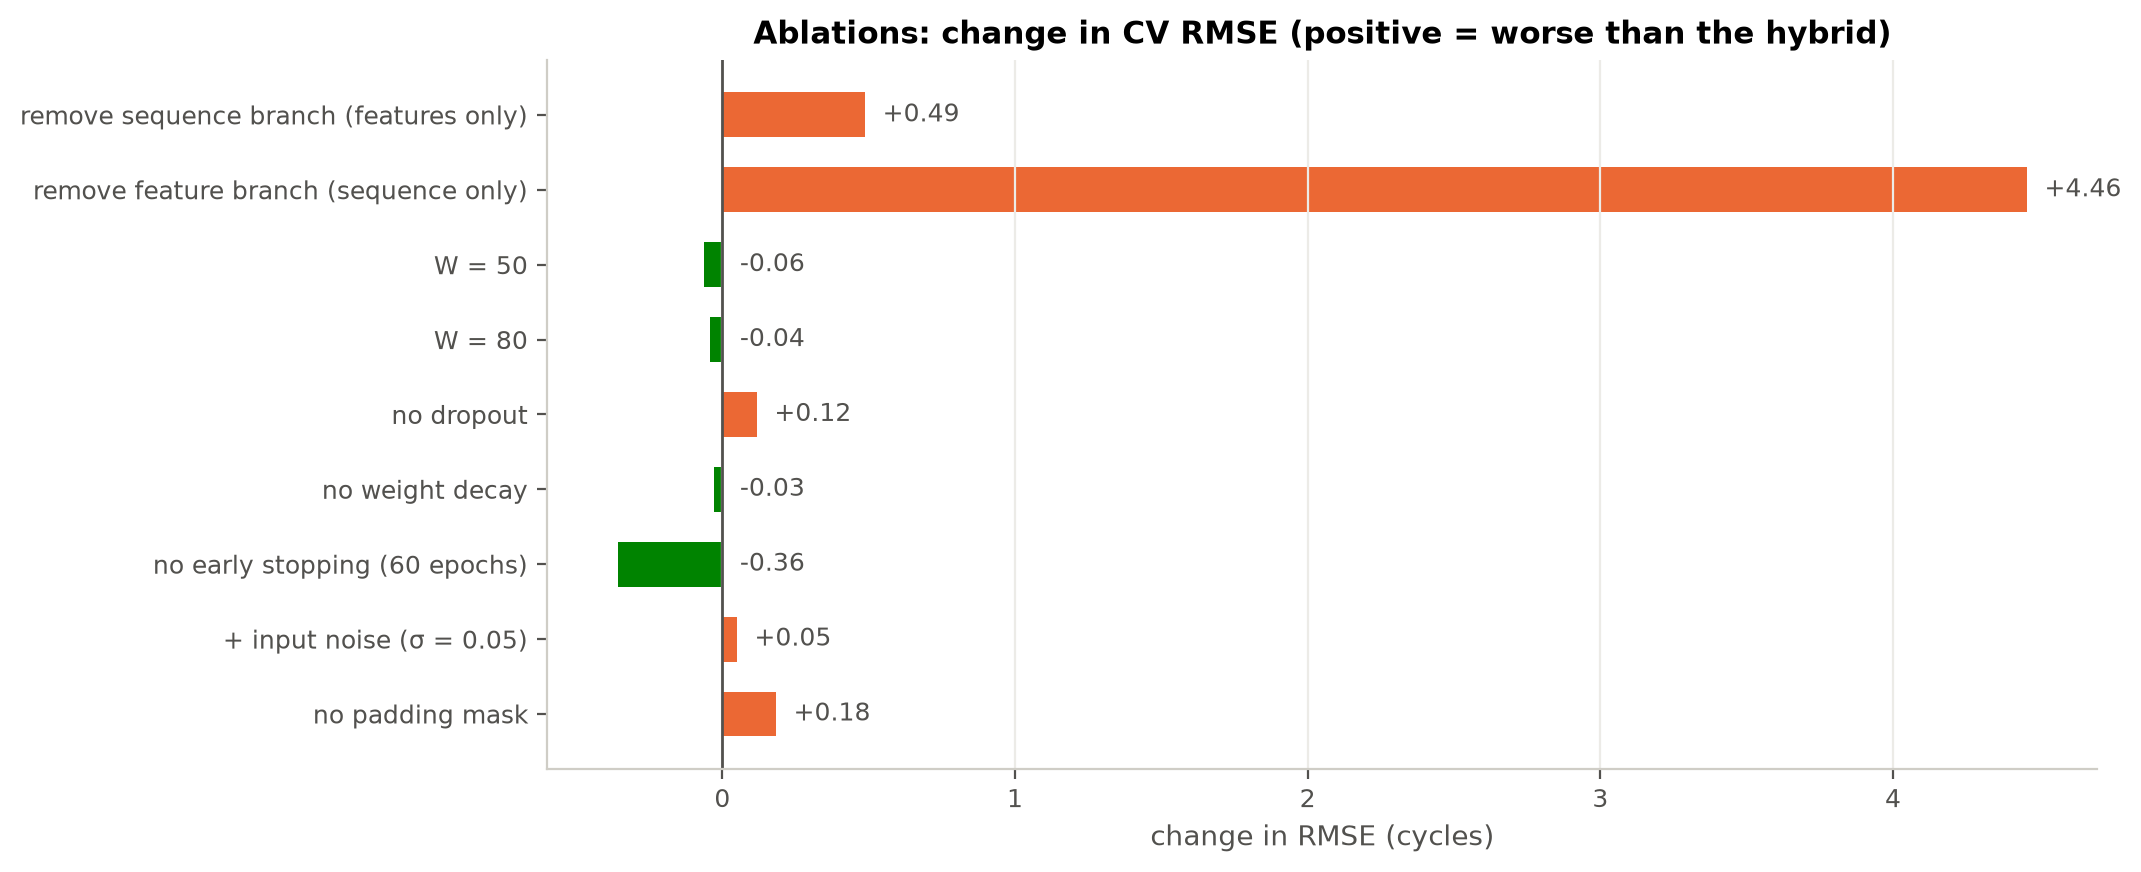
\includegraphics[width=\columnwidth]{09_ablations.png}
  \caption{Change in CV RMSE for each ablation (positive = worse). Changes below about 0.5 are within seed noise.}
  \label{fig:ablation}
\end{figure}

\begin{figure}[t]
  \centering
  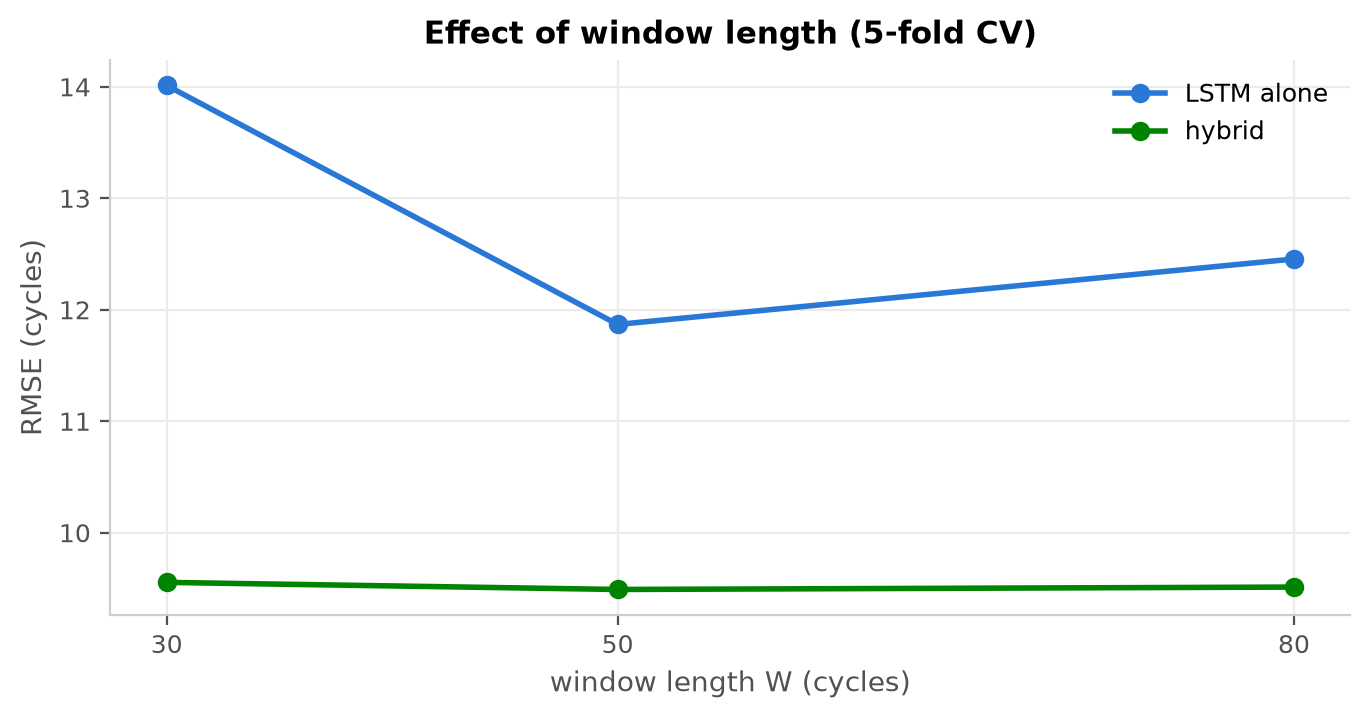
\includegraphics[width=0.8\columnwidth]{09_window_length.png}
  \caption{Window length: the sequence-only LSTM gains from longer histories; the hybrid does not need them.}
  \label{fig:window}
\end{figure}

% Section owner: Vansh Khod -- test-set validation, discussion and conclusion
\section{Test-Set Validation}\label{sec:test}
The models were retrained on all 100 training engines (10 held out for validation) with three seeds each, and evaluated once on the official test set, with the same protocol as Phase~1. The reported prediction of each network is the average of its three seeds. Phase~1's tuned XGBoost was retrained alongside so that all models are scored on identical rows.

\subsection{Official benchmark}
Table~\ref{tab:test} reports the last-cycle results against the true RUL with 95\% bootstrap intervals over engines. The hybrid scores 11.02 (9.3--12.7), level with XGBoost (10.75, 9.1--12.4), with a slightly lower MAE (8.02 vs.\ 8.09). Its three seeds score 11.05--11.68, so seed variation is of the same size as the differences between the best models. The sequence-only networks score 14.7--15.5: better than XGBoost on raw single-cycle sensors (18.19), but clearly behind the engineered features, the same ranking as in cross-validation.

\begin{table}[t]
\centering
\small
\setlength{\tabcolsep}{4pt}
\caption{Official FD001 test set (last cycle, true RUL)}
\label{tab:test}
\resizebox{\columnwidth}{!}{\begin{tabular}{lccc}
\toprule
Model & RMSE [95\% CI] & MAE & Score \\
\midrule
XGBoost, raw sensors (Ph.~1) & 18.19 [14.9, 21.2] & 12.93 & 963 \\
LSTM, sensor windows & 15.52 [13.0, 18.0] & 11.63 & 463 \\
Transformer, sensor windows & 15.03 [12.7, 17.3] & 11.17 & 367 \\
TCN, sensor windows & 14.72 [12.6, 16.7] & 11.21 & 322 \\
XGBoost, engineered (Ph.~1) & \textbf{10.75 [9.1, 12.4]} & 8.09 & \textbf{161} \\
Hybrid (LSTM + features) & 11.02 [9.3, 12.7] & \textbf{8.02} & 166 \\
\bottomrule
\end{tabular}}
\end{table}

\subsection{Significance}
Because all models are scored on the same engines, we compare them with a paired Wilcoxon signed-rank test~\cite{wilcoxon1945} on per-engine absolute errors, which does not assume normally distributed errors. Each sequence-only network is significantly worse than XGBoost ($p\leq0.0015$; better on only 33--40 of 100 engines). The hybrid and XGBoost are statistically indistinguishable ($p=0.90$; the hybrid is better on 51 engines). Their last-cycle errors are strongly correlated ($r=0.86$): the same engines are hard for both.

\subsection{Error by degradation stage}
Scoring every test cycle (13{,}096 points) against the capped target, the hybrid has a lower RMSE than XGBoost in every stage: early 5.95 vs.\ 6.44, mid 12.33 vs.\ 12.44, late 5.37 vs.\ 5.70, and 8.54 vs.\ 8.81 overall (Fig.~\ref{fig:stage}). Its late-stage bias stays small ($+2.9$ cycles), while the LSTM alone is biased late by $+6.3$ cycles near failure, the dangerous direction. At the last cycle of the 33 engines closest to failure (true RUL $\leq50$), the hybrid has the lowest MAE (2.93, vs.\ 3.38 for XGBoost and 4.39 for the LSTM). Fast-degrading engines remain about 10 cycles late for every model.

\begin{figure}[t]
  \centering
  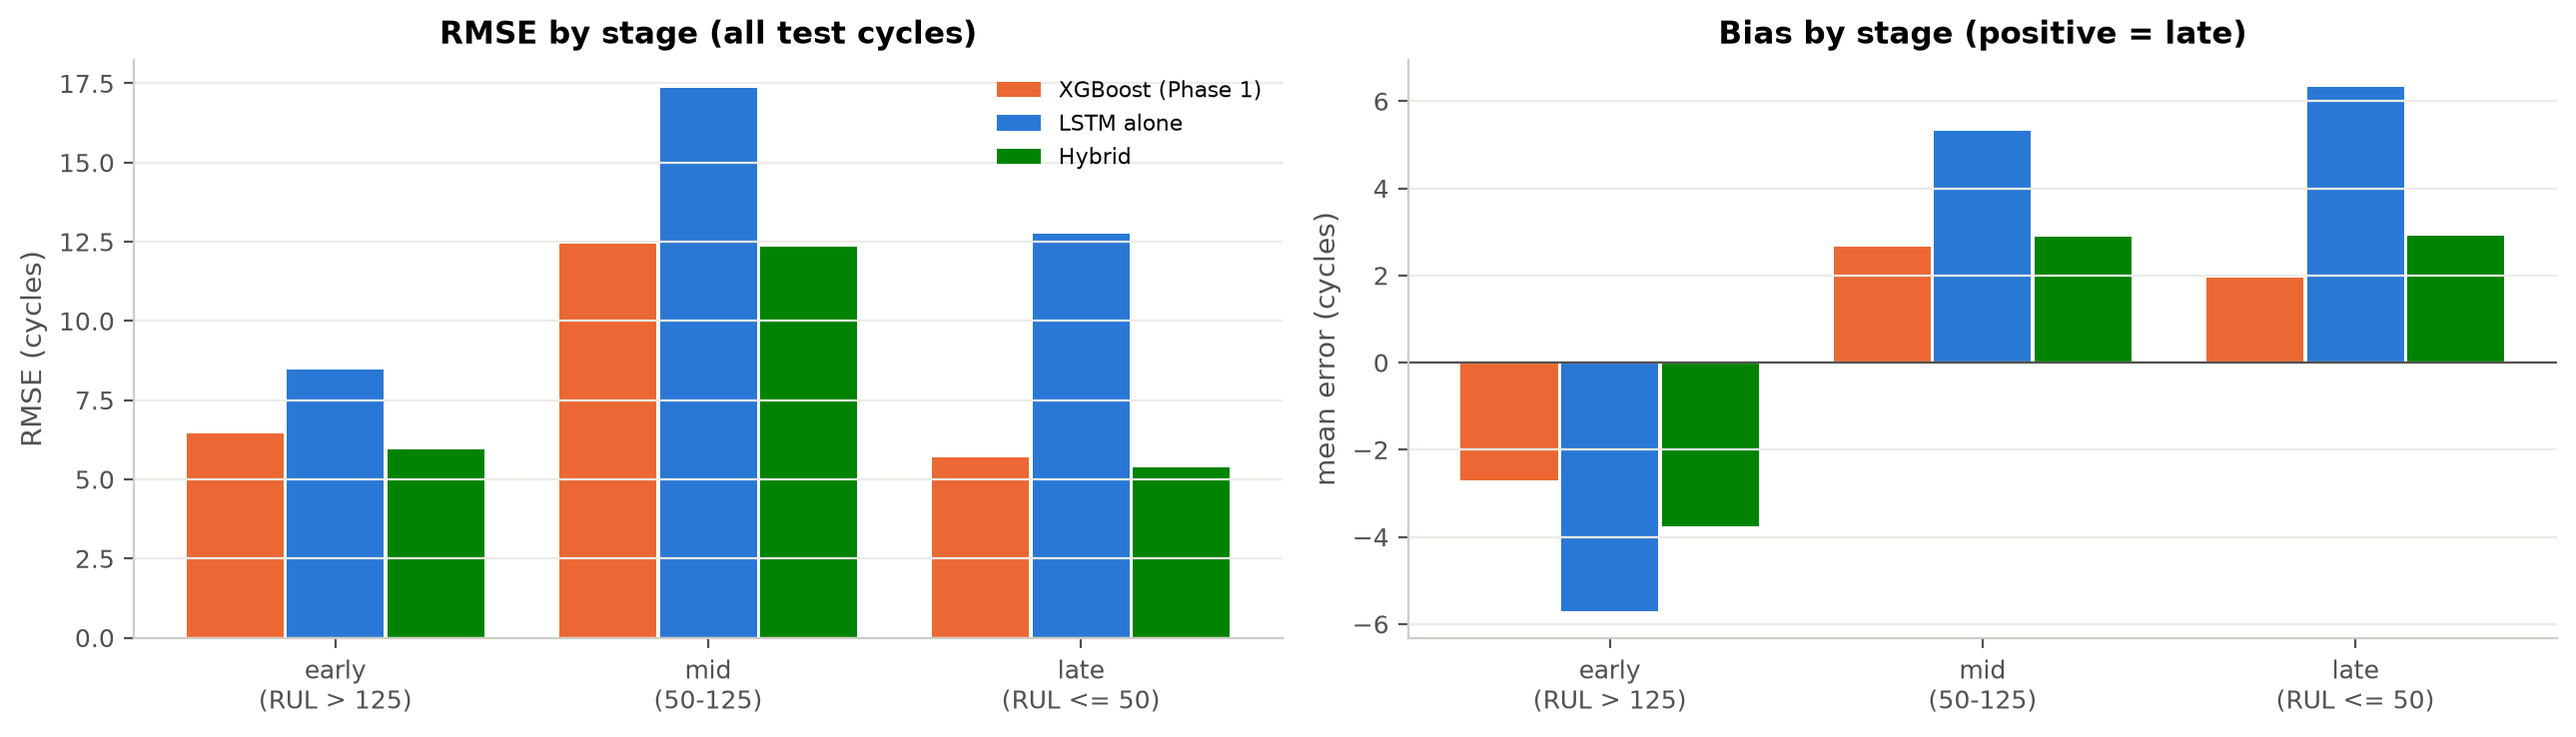
\includegraphics[width=\columnwidth]{10_error_by_stage.png}
  \caption{Test RMSE and bias by degradation stage over all test cycles.}
  \label{fig:stage}
\end{figure}

\subsection{What the sequence branch looks at}
Gradient saliency~\cite{simonyan2014saliency}, the mean $|\partial\hat y/\partial x_{s,\tau}|$ over test windows with RUL $\leq80$ (Fig.~\ref{fig:saliency}), shows that the network concentrates on the last ten or so cycles and on the core speeds $s_9$ (Nc) and $s_{14}$ (NRc), the HPC outlet pressure $s_7$ and the temperature $s_4$. The core speeds were the weakest sensors in Phase~1's ranking and carried little weight in the PCA health index. The sequence branch therefore exploits exactly the signal that the hand-made features use least, which is direct evidence of the complementarity behind the hybrid.

\begin{figure}[t]
  \centering
  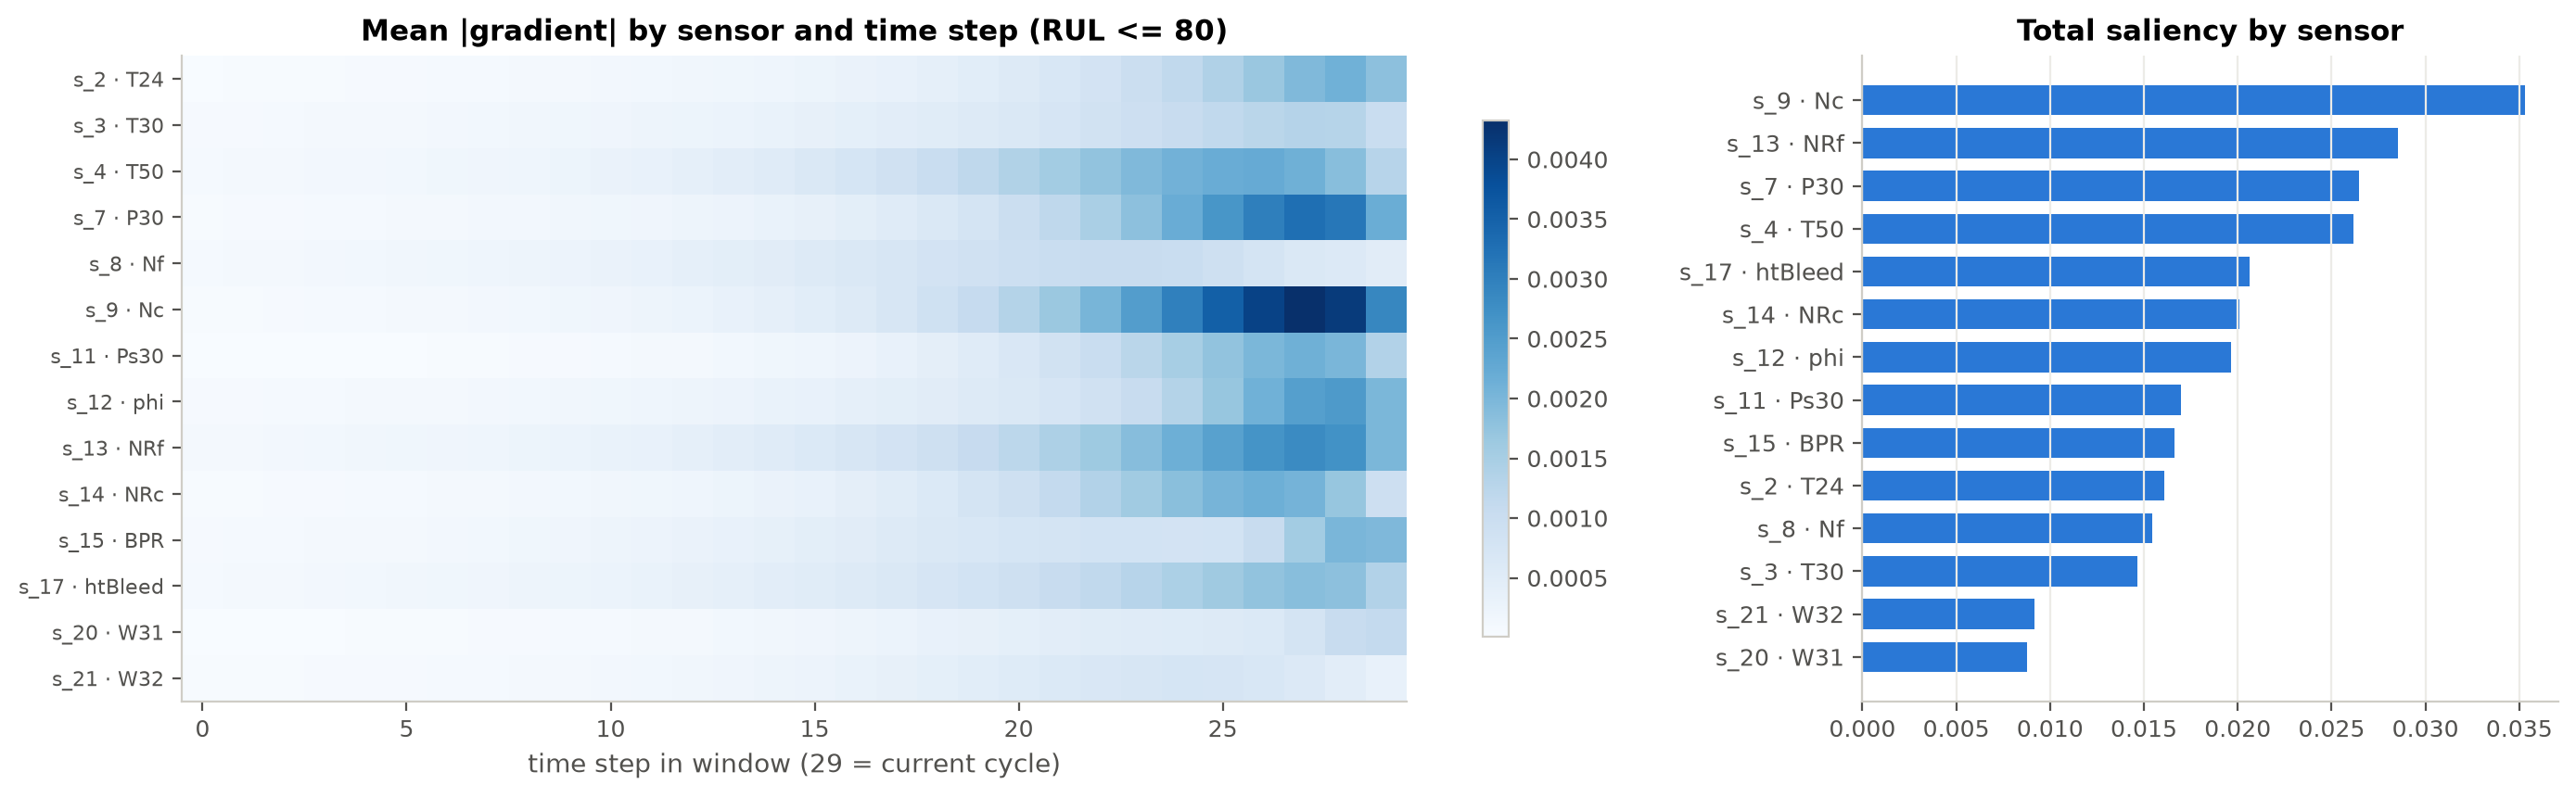
\includegraphics[width=\columnwidth]{10_saliency.png}
  \caption{Gradient saliency of the hybrid's sequence branch by sensor and time step.}
  \label{fig:saliency}
\end{figure}

\section{Discussion and Limitations}
The central comparison of the project has a clear answer on FD001: models that learn only from sensor sequences learn real degradation patterns (3--3.5 cycles better than raw single-cycle features) but do not reach carefully engineered degradation features. The reason is identified by the experiments: the most informative quantities, each engine's distance from its own healthy baseline and its age, lie outside any fixed window, and 100 engines are too few to learn such references. Longer windows help a sequence-only model (14.0 to 11.9 at $W=50$), which supports the brief's hypothesis that fixed windows miss long trajectories. Supplying the context through engineered features helps more.

The hybrid recovers the whole gap, beats both its parts and late fusion in cross-validation, and matches the best feature-based model on the official benchmark, with a small but consistent advantage over all test cycles and near failure. We do not claim a significant improvement over XGBoost: the paired test shows none.

\textbf{Limitations.} FD001 has one operating condition, one fault mode and 100 test engines, so confidence intervals are about $\pm1.7$ cycles wide. Network training is noisy: retraining with another seed moves a CV score by about $\pm0.5$--$0.7$ cycles, as large as most design effects we measured, so only larger effects are claimed. Hyperparameters of the networks were not searched as extensively as XGBoost's in Phase~1, partly for this reason, and early stopping relied on only 7--8 inner-validation engines. Saliency is a local sensitivity measure, not a causal explanation.

\textbf{Future work.} Fast-degrading engines are predicted late by every model, because all of them use the engine's age. Features or targets that express degradation \emph{rate} rather than age, and evaluation on the multi-condition subsets FD002--FD004 (our regime-normalisation pipeline already supports them), are the natural next steps.

\section{Conclusion}
We built a leakage-free sequence-learning pipeline for RUL prediction and compared an LSTM, a temporal CNN and a Transformer encoder with Phase~1's engineered-feature regression under identical engine-level protocols. On their own, the sequence models are significantly worse than the engineered features (test RMSE 14.7--15.5 vs.\ 10.75). A hybrid that fuses an LSTM encoder with the engineered degradation features closes this gap (11.02, statistically level with XGBoost), has the lowest error over all test cycles in every degradation stage, and its sequence branch draws on sensors the features under-use. On 100 engines, domain-informed degradation features remain the backbone of accurate RUL prediction, and sequence learning is most valuable as a complement to them rather than a replacement.


\section*{Team Contributions}
{\small
\begin{tabular}{p{0.25\columnwidth}p{0.6\columnwidth}}
\toprule
Member & Phase 2 responsibility \\
\midrule
Kushal Tyagi & Sequence data pipeline, leakage checks, training loop and regularisation (notebook 06, \texttt{src/sequences.py}, \texttt{src/training.py}) \\
Anant Lalwani & Deep learning literature; LSTM, TCN and Transformer architectures and their comparison (notebook 07, \texttt{src/dl\_models.py}) \\
Nishant Sharma & Hybrid feature-fusion model: rationale, design and evaluation (notebook 08, \texttt{src/hybrid.py}) \\
Dev Tyagi & Ablation studies and final configuration (notebook 09) \\
Vansh Khod & Test-set validation: seeds, bootstrap, significance, stages, saliency (notebook 10, \texttt{src/validation.py}) \\
\bottomrule
\end{tabular}}

\vspace{4pt}
\noindent Code and notebooks: \url{https://github.com/WhiteHacker000/Remaining-Useful-Life-Prediction-for-Industrial-Engines}

\bibliographystyle{IEEEtran}
\bibliography{references}

\end{document}
